% lint-skip: 未完成ステータス（figure/table caption 未対応，人手チェック時に解消予定）
\documentclass[../../main.tex]{subfiles}
\begin{document}

\begin{flushright}
  \footnotesize\textit{【自動文字起こし・要確認】}
\end{flushright}

[解] $P$の$x$座標を$t$とおくと
$$
\begin{cases}
  t^3-t=t^2-a & \cdots \text{①} \\
  3t^2-1=2t & \cdots \text{②}
\end{cases}
$$
②から $t=-\dfrac{1}{3}, 1$ だから，①に代入して
$$ (t, a) = \left(-\dfrac{1}{3}, -\dfrac{5}{27}\right), (1, 1) $$
である．以下，$f(x)=x^3-x, g(x)=x^2-a$とおく．

$1^{\circ} (t,a) = \left(-\dfrac{1}{3}, -\dfrac{5}{27}\right)$ の時
グラフは下図で
求める面積は
\begin{align}
  S &= \int_{-\frac{1}{3}}^{\frac{5}{3}} \{g(x)-f(x)\} dx \\
  &= \int_{-\frac{1}{3}}^{\frac{5}{3}} -\left(x+\dfrac{1}{3}\right)^2\left(x-\dfrac{5}{3}\right) dx \\
  &= \dfrac{1}{12} \left(\dfrac{5}{3}+\dfrac{1}{3}\right)^4 = \dfrac{4}{3}
\end{align}

\begin{figure}[H]
  \centering
  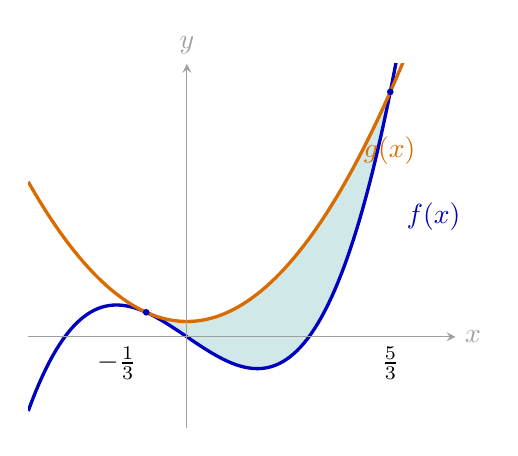
\begin{tikzpicture}[x=1.55cm,y=1.05cm,>=stealth]
    \begin{scope}
      \clip (-1.3,-1.1) rectangle (2.15,3.3);
      \fill[teal!18]
      plot[domain=-1/3:5/3,samples=90] (\x,{\x*\x+5/27})
      -- plot[domain=5/3:-1/3,samples=90] (\x,{\x*\x*\x-\x}) -- cycle;
      \draw[blue!75!black,very thick,domain=-1.3:2.1,samples=120]
      plot (\x,{\x*\x*\x-\x});
      \draw[orange!85!black,very thick,domain=-1.3:2.1,samples=90]
      plot (\x,{\x*\x+5/27});
    \end{scope}
    \draw[->,gray!75] (-1.3,0)--(2.2,0) node[right] {$x$};
    \draw[->,gray!75] (0,-1.1)--(0,3.3) node[above] {$y$};
    \fill[blue!75!black] (-1/3,{(-1/3)^3+1/3}) circle (1.2pt)
    (5/3,{(5/3)^2+5/27}) circle (1.2pt);
    \node[below left] at (-1/3,0) {$-\frac13$};
    \node[below] at (5/3,0) {$\frac53$};
    \node[blue!75!black,right] at (1.72,1.45) {$f(x)$};
    \node[orange!85!black,right] at (1.37,2.25) {$g(x)$};
  \end{tikzpicture}
  \caption{$a=-5/27$ のとき．着色部が求める面積}
\end{figure}

$2^{\circ} (t,a) = (1, 1)$ の時
グラフは下図で
\begin{align}
  S &= \int_{-1}^{1} \{f(x)-g(x)\} dx \\
  &= \int_{-1}^{1} (x-1)^2(x+1) dx \\
  &= \dfrac{4}{3}
\end{align}

\begin{figure}[H]
  \centering
  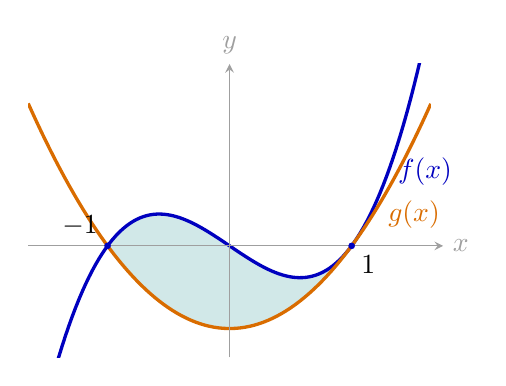
\begin{tikzpicture}[x=1.55cm,y=1.05cm,>=stealth]
    \begin{scope}
      \clip (-1.65,-1.35) rectangle (1.65,2.2);
      \fill[teal!18]
      plot[domain=-1:1,samples=90] (\x,{\x*\x*\x-\x})
      -- plot[domain=1:-1,samples=90] (\x,{\x*\x-1}) -- cycle;
      \draw[blue!75!black,very thick,domain=-1.65:1.65,samples=120]
      plot (\x,{\x*\x*\x-\x});
      \draw[orange!85!black,very thick,domain=-1.65:1.65,samples=90]
      plot (\x,{\x*\x-1});
    \end{scope}
    \draw[->,gray!75] (-1.65,0)--(1.75,0) node[right] {$x$};
    \draw[->,gray!75] (0,-1.35)--(0,2.2) node[above] {$y$};
    \fill[blue!75!black] (-1,0) circle (1.2pt) (1,0) circle (1.2pt);
    \node[above left] at (-1,0) {$-1$};
    \node[below right] at (1,0) {$1$};
    \node[blue!75!black,right] at (1.3,0.9) {$f(x)$};
    \node[orange!85!black,right] at (1.22,0.38) {$g(x)$};
  \end{tikzpicture}
  \caption{$a=1$ のとき．着色部が求める面積}
\end{figure}

以上からいずれの場合も
$$ S = \dfrac{4}{3} $$

\end{document}
